% Compile from this directory so that figures/ resolves correctly.
% pdflatex open_loop_control.tex   (run twice for references)
% Figures are separate vector PDF and SVG files; TikZ is not required.
\documentclass[11pt,letterpaper]{article}
\usepackage[T1]{fontenc}
\usepackage{lmodern}
\usepackage[margin=0.8in]{geometry}
\usepackage{amsmath,amssymb}
\usepackage{graphicx,booktabs,tabularx,array}
\usepackage{xcolor,listings,enumitem,microtype}
\usepackage{float,placeins}
\usepackage{hyperref}
\hypersetup{colorlinks=true,linkcolor=blue!45!black,urlcolor=blue!45!black,
  citecolor=blue!45!black,pdftitle={Bidirectional Open Loop Motor Control},
  pdfauthor={Laser Tracking Gimbal Project}}
\graphicspath{{figures/}}
\setlength{\parindent}{0pt}
\setlength{\parskip}{4pt}
\postdisplaypenalty=10000
\setlength{\emergencystretch}{2em}
\renewcommand{\topfraction}{0.95}
\renewcommand{\textfraction}{0.05}
\renewcommand{\floatpagefraction}{0.85}
\setlength{\textfloatsep}{12pt plus 2pt minus 2pt}
\renewcommand{\arraystretch}{1.18}
\setlist{nosep,leftmargin=1.5em,topsep=4pt}
\newcommand{\code}[1]{\texttt{\detokenize{#1}}}
\newcommand{\rpm}{\mathrm{RPM}}
\newcolumntype{Y}{>{\raggedright\arraybackslash}X}
\lstset{basicstyle=\ttfamily\small,columns=fullflexible,keepspaces=true,
  breaklines=true,showstringspaces=false,frame=none,
  aboveskip=6pt,belowskip=6pt}
\title{\textbf{Bidirectional Open Loop Motor Control}\\[4pt]
  \large Working principles and firmware implementation}
\author{Laser Tracking Gimbal Project}
\date{Firmware v0.5.0 \quad Source snapshot e0acf5c \quad 13 October 2026}

\begin{document}
\maketitle
\vspace{-1.8em}

\section{What this firmware does}

The current bench firmware drives one DFRobot FIT1036 motor from a
NUCLEO-H753ZI and BOOSTXL-DRV8304H. A potentiometer commands signed speed,
a physical RUN input authorizes operation, and the MCU generates a rotating
three-phase voltage pattern. The permanent-magnet rotor follows that pattern
when available torque, acceleration and load allow it to stay synchronized.

The implementation is \textbf{open-loop sinusoidal voltage commutation}.
Its speed value describes the generated field, not a measured shaft speed.
The 0--3 V pot commands $-100$ to $+100\,\rpm$, with a 1.3--1.7 V neutral band.
The motor bus is 24 V; the running voltage-vector command is 2 V.
The dedicated commutation module is 105 physical source lines.

\begin{figure}[H]
  \centering
  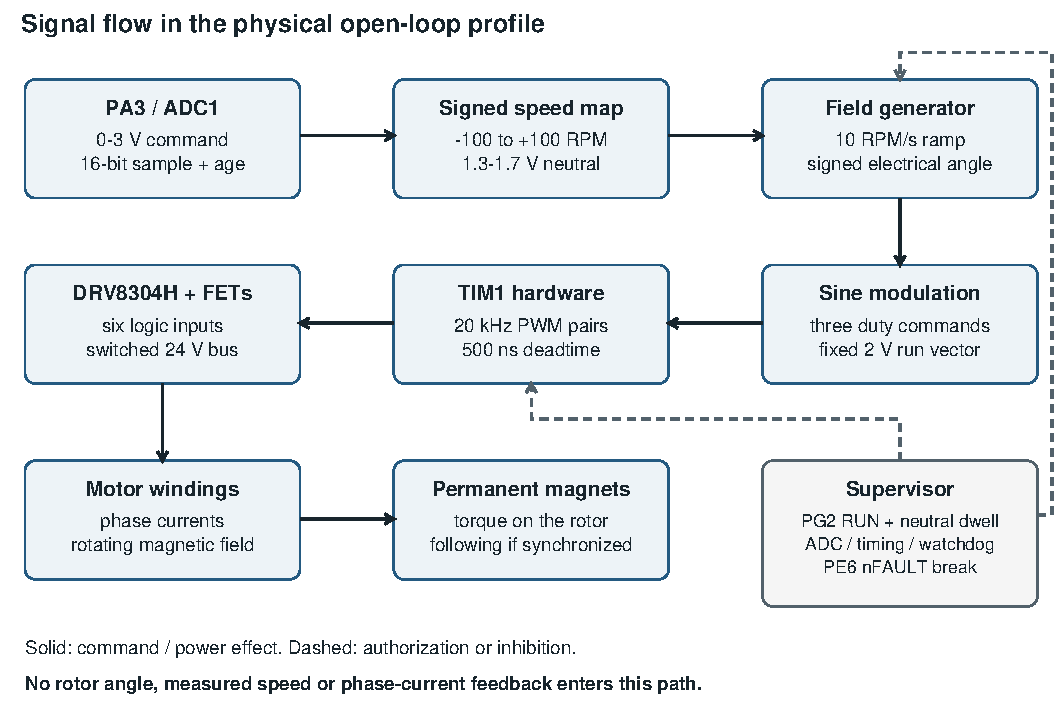
\includegraphics[width=0.94\linewidth]{01_system_flow.pdf}
  \caption{The current signal and power path. Supervision can inhibit drive;
  no motor-motion measurement closes the speed loop.}
  \label{fig:system}
\end{figure}


\section{Dependencies and the bench interface}

\subsection{Hardware required for this mode}

The Nucleo computes duties. The DRV8304H translates six 3.3 V logic inputs
into MOSFET gate drive, and the EVM's three half bridges switch the 24 V bus
into the motor windings. Motor power comes from the bench supply, not the
Nucleo. Logic and command sources share a ground reference. The FIT1036
has 11 pole pairs, or 22 rotor poles.\cite{motor,evm}

\begin{table}[H]
\centering\small
\begin{tabularx}{\linewidth}{@{}l l Y@{}}
\toprule
Function & MCU connection & Bench connection \\
\midrule
Signed speed & PA3 / A0 & CN9 pin 1 or CN12 pin 37; 0--3 V to GND \\
RUN & PG2 & CN11 pin 42; HIGH requests operation, LOW stops \\
Driver ENABLE & PG4 & CN12 pin 69 to EVM J5 pin 9; firmware output \\
Driver nFAULT & PE6 / BKIN2 & CN11 pin 62 to EVM J5 pin 15; active LOW \\
Phase A high / low & PE9 / PE8 & EVM J4 pins 1 / 3, INHA / INLA \\
Phase B high / low & PE11 / PE10 & EVM J4 pins 5 / 7, INHB / INLB \\
Phase C high / low & PE13 / PE12 & EVM J4 pins 9 / 11, INHC / INLC \\
Logic supply & Nucleo 3.3 V & EVM J5 pin 1, VDDIO; verify rail straps \\
Ground & Common GND & EVM signal reference and power return routing \\
Winding power & 24 V bench bus & EVM J1; motor A/B/C at J2 \\
Indicators & PE1 / PB14 & Nucleo yellow LD2 / red LD3 \\
\bottomrule
\end{tabularx}
\caption{Current wiring. INLB is PE10, not the former PB0 connection.
Nucleo PE10 is CN12 pin 47, also D40/CN10 pin 24.}
\end{table}

Use the DRV8304H hardware \textbf{MODE tied to AGND for 6-PWM}, with CAL low.
Hardware GAIN, IDRIVE and VDS straps must be verified on the actual EVM;
firmware does not program them. Retain an effective ENABLE pull-down and an
nFAULT pull-up to 3.3 V. The user's 4.7 kOhm RUN pull-down is suitable;
PG2 also has an internal pull-down.\cite{drv,evm,nucleo}

All three motor leads are winding terminals. A reproducible bench assignment
is red=A, black=B, yellow=C; this is an arbitrary assignment, not a verified
manufacturer color code. Physical clockwise/counterclockwise depends on this
order and the viewing side. No winding lead connects directly to supply or GND.

\textbf{Analog disconnection.} Zero volts now means full reverse.
A PA3 pull-down therefore does not give a disconnected-input stop. Equal
10 kOhm resistors to 3.3 V and GND can bias an unplugged signal near 1.65 V;
remove any former pull-down and verify the pot's loaded voltage range.
Once armed, software cannot distinguish an intentional low command from a
broken command wire held low. RUN LOW is the independent drive inhibit.

\subsection{Software required to run and build it}

The MCU runs bare-metal C using STM32H7 HAL and CMSIS, the H753 startup/vector
code and flash linker script, and the C runtime/math library. There is no RTOS
or external motor-control library in the active algorithm. Helpers use
\code{sinf}, \code{cosf}, \code{fmodf}, \code{fminf}, \code{fmaxf} and finite-value
checks. The physical profile does not start encoder transactions, a serial
console or networking. Shared board initialization still configures I2C and
USART3 hardware; those peripherals are not control dependencies or required
bench connections here.

Normal CubeIDE builds use these existing header selections:
\begin{lstlisting}[language=C]
#define DEMO_DEFAULT_OPEN_LOOP 1
#define DEMO_OPEN_BOARD_CONTROL 1
#define DEMO_PWM_SCOPE_TEST 0
\end{lstlisting}

STM32CubeIDE 1.18.0 with ARM GCC 13.3.1 was used for verification.
The optional \code{Tools/build.py} uses Python's standard library and ARM GCC;
Python is not part of the flashed runtime. Host tests additionally need a
native C compiler (Zig was used) and Python. The archived IOC is historical:
\code{board.c} owns the actual initialization and must not be overwritten by
CubeMX regeneration.

\section{From switching voltages to motor movement}

\subsection{What the inverter actually applies}

Each phase has an upper MOSFET to the positive bus and a lower MOSFET to the
negative return. Switching the pair alternately makes the phase node approximately
0 or 24 V relative to power ground. If the upper-switch duty is $D_A$, an ideal
carrier-average phase-node voltage is
\begin{equation}
  \overline{v_{A,G}}\simeq D_A V_{\mathrm{bus}}.
\end{equation}
The motor is driven by differences between its terminals, for example
\begin{equation}
  \overline{v_{AB}}\simeq (D_A-D_B)V_{\mathrm{bus}}.
  \label{eq:linevoltage}
\end{equation}
Thus all duties can stay close to 50\% while still producing positive and
negative winding excitation. The common 50\% offset cancels in a line-to-line
voltage. The motor's internal neutral, if present, is not the scope's ground.
These averages neglect deadtime, device drops and switching transients.

The code requests balanced phase-voltage references. In the active path,
\code{motor_modulate(theta, open_volts, 0, duty)} reduces to
\begin{align}
  v_A^* &= U\cos\theta_e,\\
  v_B^* &= U\cos(\theta_e-2\pi/3),\\
  v_C^* &= U\cos(\theta_e+2\pi/3),\\
  D_x &= \operatorname{clip}\!\left(\tfrac12+
               \frac{v_x^*}{24\,\mathrm{V}},\,0.05,\,0.95\right).
  \label{eq:duties}
\end{align}
Here $U$ is the commanded voltage-vector magnitude and $\theta_e$ is a
\emph{generated electrical angle}. The helper's generic $d/q$ arguments are
just a coordinate transform in this path; their frame is not locked to a
measured rotor. With $U=2\,\mathrm{V}$, ideal duties span
\textbf{41.67--58.33\%}. The line-to-line sinusoidal peak is
$\sqrt{3}U\simeq3.46\,\mathrm{V}$, while raw phase-node pulses still reach 24 V.



\begin{figure}[!ht]
  \centering
  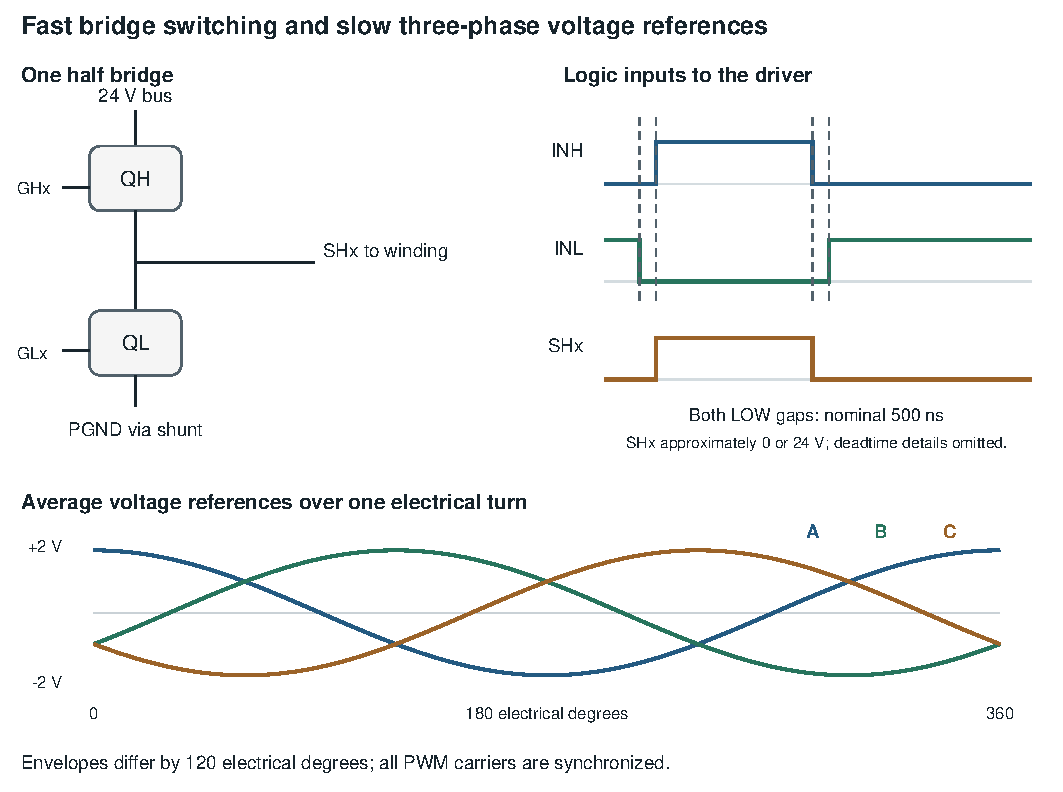
\includegraphics[width=0.94\linewidth]{03_pwm_and_phase_voltages.pdf}
  \caption{Complementary logic produces fast switching. Slowly changing,
  phase-shifted duty envelopes produce balanced voltage references. The upper
  waveforms are schematic; deadtime gaps are exaggerated.}
  \label{fig:pwm}
\end{figure}

At $\theta_e=0$ during 2 V running excitation, the phase references are
$(2,-1,-1)\,\mathrm{V}$, so duties are approximately
$(58.33,45.83,45.83)\%$. Equal B/C duty at that angle is normal.
At alignment's 1 V peak they are $(54.17,47.92,47.92)\%$.
These numbers describe pre-deadtime commands, not calibrated loaded measurements.

\subsection{Why the magnets move}

\textbf{Current creates the stator magnetic field.} PWM changes winding voltage;
inductance prevents current from following every edge instantaneously. A
simplified phase model explains the relationship:
\begin{equation}
  v = Ri + L\frac{di}{dt} + e,
\end{equation}
where $R$ is resistance, $L$ is inductance and $e$ is rotor-generated back EMF.
The resulting currents, rather than voltage alone, determine field magnitude
and direction. Current ripple and phase lag remain; PWM is not an ideal
sine-wave voltage source at each instant.

With approximately balanced sinusoidal currents in three spatially displaced
windings, their magnetic contributions combine into a rotating stator field.
The permanent-magnet rotor experiences torque when its magnetic axis is
misaligned with that field. If excitation rotates gently enough, the rotor
follows with a load-dependent angular offset.\cite{stphysics}

In an idealized sinusoidal magnet model,
\begin{equation}
  \tau \propto |B_s|\,|B_r|\sin\delta,
\end{equation}
where $B_s$ is the current-produced stator field, $B_r$ is the rotor magnet
field and $\delta$ is their angular separation. This illustrates why the
relative magnetic angle creates torque; it is not a torque estimate made by
the firmware. The imposed voltage-vector angle need not equal the actual
stator-current angle.

There is no measurement that confirms this following. Excessive load,
acceleration or back EMF can cause loss of synchronization, jerking or stall
while PWM continues. A 2 V command is \emph{not} a current limit: current also
depends on winding parameters, speed and switching conditions. At stall or
low speed there can be sustained heating even with little shaft movement.

\subsection{Electrical angle and mechanical angle}

For $p=11$ pole pairs, the field completes eleven electrical cycles for one
synchronous shaft revolution:
\begin{equation}
  \omega_e=p\omega_m,\qquad f_e=\frac{p\,n}{60}.
  \label{eq:electrical}
\end{equation}
One electrical revolution corresponds to about $32.73^\circ$ of mechanical
rotation. At $100\,\rpm$, the electrical pattern runs at $18.333\,\mathrm{Hz}$,
not 100 Hz and not the 20 kHz switching carrier. Changing the sign of angle
advance reverses phase progression. Fixed-angle alignment can first move the
shaft briefly in either direction toward a nearby magnetic orientation.

\section{How the pot controls speed and direction}

\subsection{ADC conversion and signed command}

ADC1 samples PA3 in 16-bit single-ended mode. The application converts the
latest completed conversion using the configured reference:
\begin{equation}
  V_{\mathrm{pot}}=\mathrm{ADC}_{\mathrm{raw}}
                       \frac{3.3\,\mathrm{V}}{65535}.
\end{equation}
A conversion is software-triggered asynchronously near the end of each control
tick; the next tick normally consumes the completed sample. There is no ADC
DMA or PWM-synchronized current sampling in this mode. ADC calibration runs
at boot. Actual VDDA and source impedance affect accuracy; neutral decisions
use the converted voltage, not an independent voltage measurement.

For a valid input $0\le V\le3.15\,\mathrm{V}$, with voltage expressed in volts,
\begin{equation}
 n^*(V)=
 \begin{cases}
  100\,(V-1.3)/1.3, & 0\le V<1.3,\\
  0, & 1.3\le V\le1.7,\\
  100\,\min\!\big((V-1.7)/1.3,1\big), & 1.7<V\le3.15.
 \end{cases}
 \label{eq:map}
\end{equation}
Values above 3.15 V are invalid in firmware; negative/nonfinite inputs are
also rejected by the portable mapping helper. This software bound does not
replace PA3 electrical input limits.

\begin{figure}[!ht]
  \centering
  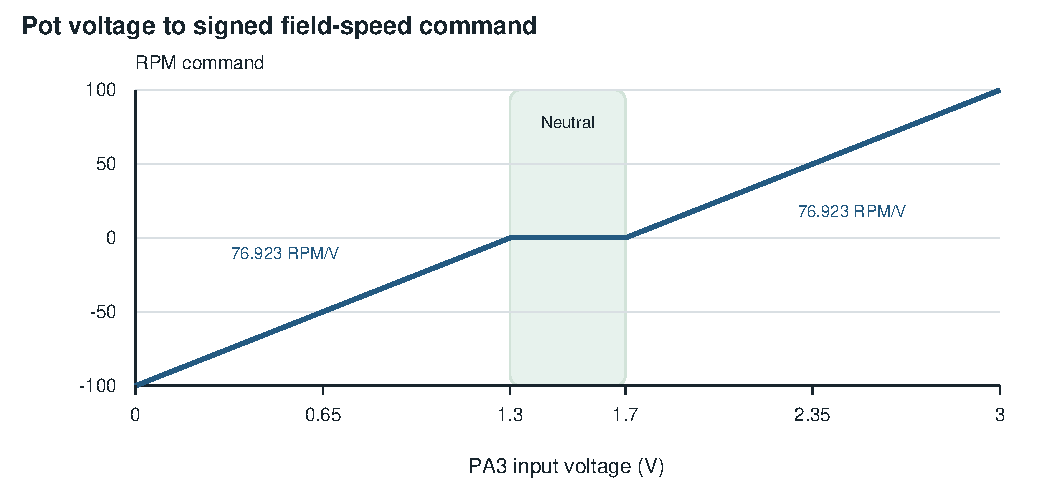
\includegraphics[width=0.94\linewidth]{04_analog_speed_map.pdf}
  \caption{Symmetric command mapping. The shaded center band is stationary
  command and the only permitted initial arming region.}
\end{figure}

\begin{table}[H]
\centering\small
\begin{tabular}{@{}rrrrrrr@{}}
\toprule
Input (V) & 0 & 0.65 & 1.3--1.7 & 2.35 & 3.0 & 3.0--3.15 \\
Command (RPM) & $-100$ & $-50$ & 0 & $+50$ & $+100$ & $+100$ \\
\bottomrule
\end{tabular}
\end{table}

Each active side spans 1.3 V, giving $76.923\,\rpm/\mathrm{V}$, or 2.308 times
the previous unidirectional sensitivity. A reported 40 mV minimum now requests
about $-96.92\,\rpm$. It is not a zero-speed input. The center band has no
additional filtering or hysteresis; the initial neutral dwell is a separate
startup qualification.

\subsection{Ramp and electrical angle accumulation}

The code converts mechanical RPM to radians per second with $2\pi/60$.
During normal running, the speed reference approaches its target at
$10\,\rpm/\mathrm{s}$. At the nominal 1 ms control interval, its maximum change
is $0.01\,\rpm$ per tick. Electrical angle then advances according to
\begin{equation}
 \theta_e[k+1]=\operatorname{wrap}_{[0,2\pi)}
 \left(\theta_e[k]+11\,\omega_{m,\mathrm{ref}}[k+1]\,0.001\right).
 \label{eq:angle}
\end{equation}

For example, 2.35 V requests $+50\,\rpm$. After alignment, reaching that
reference takes about 5 s. At steady reference, $\omega_m=5.236\,\mathrm{rad/s}$,
$f_e=9.167\,\mathrm{Hz}$ and each tick advances the field by about
$0.0576\,\mathrm{rad}$ or $3.3^\circ$ electrical.

\textbf{Frequency sets commanded speed; voltage sets excitation strength.}
The pot does not scale the running magnitude: it remains 2 V after its
startup slew. A higher command makes the same duty envelope traverse its cycle
faster. The 20 kHz carrier stays fixed. A fixed 2 V may become insufficient
at higher back EMF or load; the code does not automatically compensate.
The general generated-angle principle is also described in
SimpleFOC's open-loop documentation; this firmware does not depend on that
library.\cite{simplefoc}

\section{How TIM1 produces the six PWM signals}

The clock setup uses HSI and PLL1 for a nominal 200 MHz CPU, 100 MHz AHB,
50 MHz APB clocks and 100 MHz timer kernels. TIM1 counts up and down with
prescaler zero and ARR=2500, producing
\begin{equation}
  f_{\mathrm{PWM}}=\frac{100\,\mathrm{MHz}}{2\cdot2500}
                 =20\,\mathrm{kHz},\qquad T_{\mathrm{PWM}}=50\,\mu\mathrm{s}.
\end{equation}
CH1/CH1N, CH2/CH2N and CH3/CH3N form the three complementary pairs. Only three
duties are computed; the timer derives their low-side partners. A deadtime
setting of 50 timer ticks requests nominal $500\,\mathrm{ns}$ with both
members LOW at transitions. Gate-driver delays and MOSFET behavior mean actual
gate non-overlap must be measured, not assumed from this number.\cite{drv}

\code{board_apply()} writes CCR1/CCR2/CCR3 as duty times ARR while briefly
suppressing timer update events. The three preload values become active
together at a natural carrier update. The 1 kHz control tick therefore changes
the duty references about once per twenty PWM periods. Firmware does not
bit-bang each gate edge and does not run the motor algorithm at 20 kHz.

All phases share one synchronized carrier. The \textbf{slow phase-voltage
references} are 120 electrical degrees apart; raw carrier edges are not three
independent square waves staggered by 120 degrees. At full-scale speed,
120 degrees of envelope shift is about 18.18 ms.

\textbf{Inhibit versus zero voltage.} Three active 50\% duties would request
zero ideal line-to-line average voltage but would still switch the bridge.
This firmware instead clears TIM1's main-output enable (MOE) and lowers PG4
when drive is inhibited. MOSFET body-diode/freewheel currents can still exist;
turning gates off does not force winding current or shaft velocity instantly
to zero. In 6-PWM mode the intended both-LOW input gap requests high impedance;
the code does not rely on simultaneous HIGH commands.\cite{drv}



\section{Startup authorization and alignment}

\begin{figure}[!ht]
  \centering
  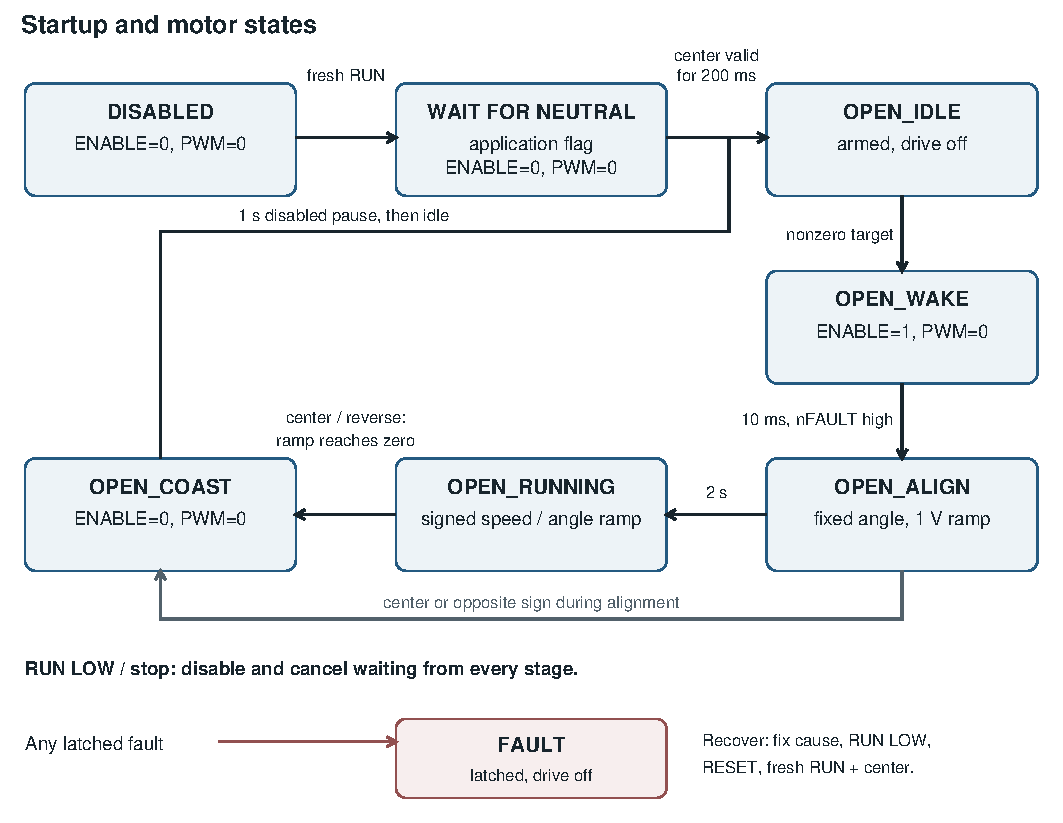
\includegraphics[width=0.94\linewidth]{02_state_machine.pdf}
  \caption{Application authorization and motor states. WAIT FOR NEUTRAL is
  an application flag while the motor remains DISABLED; it is not a separate
  member of the motor-state enum. Ordinary transitions are evaluated at 1 kHz.}
  \label{fig:states}
\end{figure}

\subsection{RUN must be deliberate and the pot must reach center}

At reset, ENABLE and PWM are inhibited. RUN must be observed LOW continuously
for at least 20 ms, then HIGH continuously for at least 20 ms. A pin already
HIGH at boot never creates an arm request: it must first go LOW and then HIGH.
A raw sampled LOW stops without waiting for debounce; the 20 ms rule governs
restart authorization.

A valid RUN request made with the pot outside neutral is retained as a pending
request, with gates off. PA3 must stay in 1.3--1.7 V continuously for 200 ms,
with valid ADC data no older than 20 ms and foreground activity no older than
100 ms. Leaving the band or losing freshness restarts that dwell.
RUN LOW, stop or a fault cancels the request. No extra RUN edge is needed just
because the original request was made outside neutral.

Yellow LD2 blinks at 2 Hz while waiting, then stays steady when armed.
In OPEN\_IDLE the bridge is still off. Moving outside center starts excitation.
Returning to center after ordinary running does not revoke RUN authorization;
a later nonzero command can start again after the stop/coast sequence.

\subsection{Wake and fixed-field alignment}

OPEN\_WAKE raises ENABLE but keeps PWM inhibited for at least 10 ms. nFAULT
must then be HIGH before alignment. Its expected wake/sleep assertion must not
be mistaken for a fresh active-drive fault; the hardware break remains present,
while break interrupt reporting is enabled only when drive is authorized.

OPEN\_ALIGN holds $\theta_e=0$ and raises $U$ linearly from 0 to 1 V over
0.5 s, within a total 2 s stage. This gives the rotor time to settle toward a
nearby orientation before the field begins rotating. No encoder confirms
success. The same fixed alignment is used for either requested direction;
direction selects subsequent angle advance. Entering neutral or changing sign
during alignment disables excitation and enters the coast pause.

OPEN\_RUNNING starts its speed ramp from zero. Voltage approaches 2 V at
2 V/s, normally taking about 0.5 s from alignment's 1 V endpoint. Full-scale
startup therefore takes roughly 10 ms wake + 2 s alignment + 10 s speed ramp,
after arming. Firmware never needs to guess a six-step sector from a stopped
back-EMF signal; it establishes a stationary field and moves it gradually.

\section{Center stop and direction reversal}

A center command requests zero reference speed. The running reference ramps
toward zero at 10 RPM/s while excitation continues. When the generated speed
reaches zero, ENABLE and PWM are inhibited for a 1 s OPEN\_COAST pause.
The controller then returns to armed OPEN\_IDLE. From 100 RPM, the generated
ramp alone takes about 10 s. Center is \textbf{not an energized position hold},
and this is not a measured braking-speed trajectory.

For opposite-direction input, the current direction is retained while the ramp
target is temporarily set to zero. After reaching zero, the bridge is disabled
for 1 s. The latest target then starts a fresh wake and alignment before
accelerating with the opposite sign. If the opposite command is withdrawn
before the reference reaches zero, the original direction can resume without
a restart. The sequence never advances the running reference directly through
zero into the opposite sign.

\begin{figure}[!ht]
  \centering
  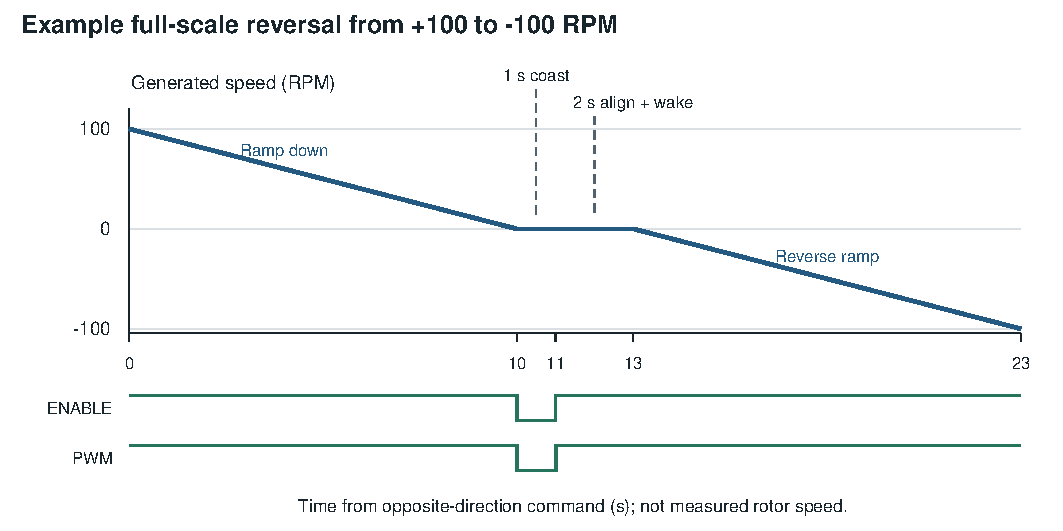
\includegraphics[width=0.94\linewidth]{05_reversal_timing.pdf}
  \caption{Approximate full-scale reference reversal. Alignment has energized
  PWM at zero generated speed. Wake is only 10 ms and is barely visible here.}
\end{figure}

A $+100$ to $-100\,\rpm$ request takes about 10 s down + 1 s disabled + 2 s
alignment + 10 s up, plus wake/control-tick timing. Yellow LD2 remains steady
because authorization is still active. RUN LOW inhibits from any stage on the
next nominal 1 ms sample; \code{board_apply()} also checks the pin immediately
before applying output authorization.

\textbf{The one-second pause does not prove standstill.} The actual rotor can
lag the reference, coast, stall or continue turning into alignment. This pause
is a configurable bench assumption, not an encoder-based reversal interlock.
Validate reversal at low speeds and inspect current and motion before using
full-scale reversals.

\section{Firmware execution and protection ownership}

\subsection{What runs at each time scale}

\begin{table}[H]
\centering\small
\begin{tabularx}{\linewidth}{@{}l l Y@{}}
\toprule
Mechanism & Nominal rate & Job \\
\midrule
TIM1 hardware & 20 kHz & Carrier edges, complementary outputs, deadtime \\
TIM7 interrupt & 1 kHz & Input snapshot, RUN/neutral logic, motor state,
angle/duty update, output authorization, next ADC request \\
ADC interrupt & Per completed sample & Publish voltage sample, validity and timestamp \\
Foreground loop & As CPU permits & Publish liveness, update LEDs, conditionally feed watchdog \\
TIM2 counter & 1 MHz & Microsecond timing measurements \\
SysTick & 1 kHz & Millisecond time for stages, debounce and sample ages \\
BKIN2 hardware / IRQ & Asynchronous & Inhibit PWM on nFAULT, then latch software fault \\
\bottomrule
\end{tabularx}
\end{table}

The commutation equations use a fixed nominal 0.001 s step. The application
measures interrupt spacing and faults if it is outside 700--1500 microseconds;
it does not substitute measured interval into angle integration. Measured
control execution above 500 microseconds also trips a fault. Thus the timer
and clock assumptions matter to commanded speed accuracy. No printf,
network polling or blocking peripheral transaction is needed in the active
control interrupt.

\begin{minipage}{\linewidth}
In execution order, the key path is:
\begin{lstlisting}
main -> board_init -> app_init -> start TIM7 / watchdog
foreground -> app_foreground (LEDs, liveness, watchdog)
TIM7 -> app_control_tick
  snapshot ADC / faults; convert volts; qualify RUN / neutral
  motor_step -> motor_open_step -> motor_modulate
  board_apply -> interlocks, ENABLE, CCR preloads, MOE
  board_sensor_tick -> next ADC conversion
\end{lstlisting}
\end{minipage}

The watchdog is refreshed at roughly 20 ms intervals only when a control tick
has occurred within the last 20 ms. IWDG uses LSI/32 and reload 999, giving a
nominal approximately 1 s reset interval; oscillator tolerance applies.
Interrupt-masked snapshots keep shared sample/action data coherent.

\subsection{Protection that remains active}

\begin{itemize}
\item \textbf{Driver fault:} PE6 feeds active-LOW TIM1 BKIN2. Hardware clears
PWM authorization independently of the control loop. The break handler latches
a board fault and lowers ENABLE; automatic output restart is disabled.
\item \textbf{ADC and foreground:} Armed idle, wake, alignment, run and coast
retain age/validity checks. Active invalid/stale ADC faults; foreground age
over 100 ms faults. While only waiting to arm, loss of freshness instead
restarts the neutral dwell with drive still off.
\item \textbf{Timing and internal failure:} Control-period/execution violations
trip inhibition. CPU fault handlers and initialization failure inhibit and
stop execution; the watchdog provides reset recovery once running.
\item \textbf{Stop and fault latches:} A RUN LOW disables independently of the
pot command. A latched fault is not cleared by nFAULT returning HIGH, moving
the pot or toggling RUN. The physical profile requires fixing the cause,
RUN LOW, RESET and a fresh RUN/neutral sequence.
\end{itemize}

These mechanisms do not regulate phase current or detect actual shaft stall,
travel or speed. Driver protection thresholds depend on EVM hardware straps.
Current-limited bench power is still needed; bus current limiting is not a
calibrated phase-current limit and can collapse the bus into undervoltage.

\section{How much code is involved}

Counts below are physical lines in source snapshot
\href{https://github.com/aaronhyzhang/lasertrackinggimbal-ece445/commit/e0acf5c962c5c35e43c126dc870b25a3903abaed}{e0acf5c}.
They include comments, blank lines and preprocessor branches, not executable
statements. Shared files include other dormant functionality; the table does
not claim every listed line executes in this profile. Vendor HAL/CMSIS,
startup assembly, linker scripts, tests and build tools are excluded from this
source subtotal.

\begin{table}[H]
\centering\small
\begin{tabularx}{\linewidth}{@{}l r Y@{}}
\toprule
File or group & Lines & Role used by this profile \\
\midrule
\code{open_loop.c} & 105 & Signed map, ramps, generated angle, alignment/coast states \\
\code{run_switch.h} & 25 & Stable LOW/HIGH request qualification; immediate sampled stop \\
\code{demo_app.c} & 207 & Input integration, neutral wait/dwell, timing, status and LEDs \\
\code{board.c} & 297 & Clocks, GPIO, ADC, timers, bridge authorization, fault/watchdog \\
\code{motor_control.c} & 197 & Dispatch, initialization, wrapping, sine modulation and faults \\
\code{main.c} & 35 & Initialization and physical-profile foreground loop \\
\code{stm32h7xx_it.c} & 20 & Timer, ADC, SysTick and CPU exception handlers \\
\code{stm32h7xx_hal_msp.c} & 3 & HAL system configuration clock setup \\
Five shared headers & 176 & Config, board/app interfaces, motor types and internal helpers \\
\midrule
\textbf{Listed source inventory} & \textbf{1065} & 13 hand-owned C/header files \\
\bottomrule
\end{tabularx}
\caption{The 105-line motor path plus 25-line RUN qualifier is the dedicated
core. Integration and hardware support make it a working bench application.}
\end{table}

The five shared headers are \code{demo_config.h} (56),
\code{motor_control.h} (58), \code{board.h} (29), \code{demo_app.h} (25) and
\code{motor_internal.h} (8). The dedicated motor and physical-application test
files contain another 160 and 120 lines respectively, totaling 280 test lines.
Counts are supplied separately in \code{source_counts.json}.

\subsection{Build footprint and dependencies}

The existing physical-profile standalone builds occupy 62,868 bytes of flash
in Debug and 37,684 bytes in Release (about 61.4 and 36.8 KiB). Reported D1
allocation is 10,392 / 10,400 bytes, including linker stack/heap reservations;
it is not a measured peak RAM or stack-use result. This profile has no
Ethernet DMA-pool allocation. These sizes include linked vendor/runtime
support and retained shared code, so they cannot be inferred from 105 lines.
The link uses function/data sections and garbage collection, but the build
source manifest still compiles the broader project.\cite{evidence}

\textbf{Useful reading order in the code:}
\code{demo_config.h}, \code{run_switch.h}, \code{open_loop.c},
the shared \code{motor_modulate()} helper, \code{app_control_tick()}, then
\code{pwm_init()} and \code{board_apply()}. This follows the command from
its configuration to physical output.

\subsection{Configuration that changes behavior}

\begin{table}[H]
\centering\small
\begin{tabularx}{\linewidth}{@{}l l Y@{}}
\toprule
Symbol in \code{demo_config.h} & Default & Meaning \\
\midrule
\code{DEMO_OPEN_MAX_RPM} & 100 & Symmetric command magnitude \\
\code{DEMO_OPEN_NEUTRAL_LOW} & 1.3 V & Lower neutral bound \\
\code{DEMO_OPEN_NEUTRAL_HIGH} & 1.7 V & Upper neutral bound \\
\code{DEMO_OPEN_NEUTRAL_DWELL_MS} & 200 ms & Continuous initial neutral qualification \\
\code{DEMO_OPEN_ACCEL_RPM_S} & 10 & Acceleration/deceleration in RPM/s \\
\code{DEMO_OPEN_COAST_MS} & 1000 ms & Disabled pause before restart \\
\code{DEMO_ALIGN_VOLTS} & 1 V & Fixed-field alignment magnitude \\
\code{DEMO_OPEN_ALIGN_RAMP_MS} & 500 ms & Alignment-voltage ramp duration \\
\code{DEMO_OPEN_ALIGN_MS} & 2000 ms & Total alignment stage \\
\code{DEMO_OPEN_VOLTS} & 2 V & Running vector magnitude \\
\code{DEMO_OPEN_VOLT_SLEW} & 2 V/s & Running voltage slew \\
\code{DEMO_POLE_PAIRS} & 11 & Electrical/mechanical angle multiplier \\
\code{DEMO_BUS_VOLTS} & 24 V & Modulation scaling; not a measured bus value \\
\code{DEMO_ADC_VREF} & 3.3 V & ADC raw-to-volts scaling \\
\code{DEMO_PWM_ARR} & 2500 & TIM1 carrier period setting \\
\bottomrule
\end{tabularx}
\end{table}

The driver wake delay is currently 10 ms in \code{open_loop.c}; it is not a
separate configuration macro. Changing PWM ARR alone does not change the
clock, deadtime or nominal control step. Review dependent settings together.
Increasing voltage is not equivalent to increasing the speed ceiling and can
increase current substantially.

\section{What has been proven and what to verify next}

The user reports that the motor spins and that the preceding 100 RPM range
looks good. Software tests pass for the new signed map, angle wrapping,
neutral ARM rules, both reversal directions, coast/re-alignment, full-speed
center stop, ADC/foreground freshness, waiting-request cancellation,
boot-HIGH inhibition, latched faults and timestamp wrap.
Configured open-loop Debug/Release and active native CubeIDE Debug/Release
builds pass; native builds report zero errors and warnings. The build record
identifies source and binary hashes. No agent hardware flash or physical
validation of the new bidirectional behavior has been performed.\cite{evidence}

A focused bench demonstration should establish these behaviors:
\begin{enumerate}
\item With windings disconnected, check the six logic inputs, complementary
pairing, actual gate-to-source non-overlap, inhibition and nFAULT shutdown.
All grounded probe clips go to the same appropriate ground reference, never
to a phase node. A high-side gate measurement is GH minus SH, not GH to GND.
\item Start with the pot at each extreme. After a fresh RUN request, gates
must stay off until an uninterrupted 200 ms center visit; brief center visits
must not arm. Confirm RUN LOW cancels waiting and boot-HIGH RUN does not arm.
\item On a secured unloaded motor, arm at center and try about 1.83 V
($+10\,\rpm$) and 1.17 V ($-10\,\rpm$). Observe alignment, direction, current,
heating and smooth following before raising speed.
\item Check center deceleration/coast and RUN LOW inhibition separately.
Try low-speed reversal and confirm the disabled pause and fresh alignment.
Measure actual shaft speed independently; a faster duty envelope alone does
not prove the rotor follows.
\end{enumerate}

The present demonstration validates generated commutation, physical control
and power-stage operation. It does not establish regulated speed, position
holding, calibrated torque/current or safe reversal under arbitrary inertia.
Those limits follow directly from the missing motion/current measurements,
not from the nominal PWM or RPM settings.

\FloatBarrier
\begin{thebibliography}{9}
\small
\bibitem{source} Project implementation, firmware v0.5.0,
\href{https://github.com/aaronhyzhang/lasertrackinggimbal-ece445/tree/e0acf5c962c5c35e43c126dc870b25a3903abaed/firmware/Senior_Design_DEV_FW}{source snapshot e0acf5c}.
All configuration values, formulas, state transitions and source counts above
are traced to this implementation unless a vendor reference is given.
\bibitem{evidence} Project
\href{https://github.com/aaronhyzhang/lasertrackinggimbal-ece445/blob/e0acf5c962c5c35e43c126dc870b25a3903abaed/firmware/Senior_Design_DEV_FW/docs/build_evidence.json}{build evidence}
and
\href{https://github.com/aaronhyzhang/lasertrackinggimbal-ece445/blob/e0acf5c962c5c35e43c126dc870b25a3903abaed/firmware/Senior_Design_DEV_FW/docs/VALIDATION.md}{validation record},
13 October 2026. Software verification and user-reported bench observations.
\bibitem{motor} DFRobot,
\href{https://wiki.dfrobot.com/fit1036/}{FIT1036 motor documentation}:
24 V bench compatibility and 11 pole pairs.
\bibitem{drv} Texas Instruments,
\href{https://www.ti.com/lit/ds/symlink/drv8304.pdf}{DRV8304 datasheet},
section 7.3.1.1.1 and Table 2: hardware MODE=AGND, 6-PWM states,
gate-drive and protection behavior.
\bibitem{evm} Texas Instruments,
\href{https://www.ti.com/lit/ug/slvub97/slvub97.pdf}{BOOSTXL-DRV8304H EVM guide},
SLVUB97: power-stage connections and header assignments.
\bibitem{nucleo} STMicroelectronics,
\href{https://www.st.com/resource/en/user_manual/um2407-stm32h7-nucleo144-boards-mb1364-stmicroelectronics.pdf}{UM2407 Nucleo board manual},
Table 22: morpho connectors and MCU pin locations.
\bibitem{stphysics} STMicroelectronics,
\href{https://www.st.com/resource/en/application_note/cd00110782-low-cost-sinusoidal-control-of-bldc-motors-with-hall-sensors-using-st7fmc-stmicroelectronics.pdf}{Low cost sinusoidal control of BLDC motors},
physical explanation of three-phase stator excitation and synchronization.
The sensor-driven implementation in that note is not a software dependency here.
\bibitem{simplefoc} SimpleFOC,
\href{https://docs.simplefoc.com/velocity_openloop}{Velocity open-loop control}:
generated-angle integration and open-loop limitations. This project uses its
own C implementation and fixed nominal control interval.
\end{thebibliography}

\end{document}
